Throughout this course we were given the task of continuously improving and adding features to a legacy code base. The code base in question was an aging mini version of Twitter called \textit{MiniTwit}.

\section*{Technologies}

\subsection*{Refactoring}

MiniTwit was originally written in Python 2 using Flask. The goal was to get the website running on a modern framework, this was done by firstly using the library 2to3, which converts Python 2 code into Python 3 code. Lastly to complete the refactoring we rewrote the code to run using the Django framework.

\subsection*{Containerization}

Containerization is a term in software development, which references to bundling application components into container images, which can then be run in isolation on a machine. To implement this technology we decided to use Docker. Using containerization solves the issues of manually installing dependencies and issues with running an application on different operating systems. By containerizing our application, the environment used locally closely resembles the environment on our production server.

\subsection*{Continuous Integration and Continuous Deployment}

DevOps is a development method where the time from the testing environment to production is rapidly shortened using automation to ensure high quality. Since we are using GitHub as our version control tool, we can use its features for testing before deploying. GitHub has a built in CI/CD tool where you can build a pipeline of checks that must be completed for the branches to be merged.

\subsection*{Cloud}

Since we are creating a web app, we need to host it somewhere. We used an Infrastructure-as-a-Service (IaaS) provider called Digital Ocean, due to it being the recommend provider from the course. Digital Ocean allowed us to create multiple server instances (Droplets), to allow for both horizontal and vertical scaling.

\subsection*{Monitoring}

Monitoring is the act of getting information about the system. An important aspect of monitoring is choosing what to monitor, since it does not make sense to log and measure every part of the system, because this would take an unreasonable amount of space and complexity. Therefore, you need to be selective with what metrics you monitor, to give only the insights you require. This can be anything from the technical aspect of uptime/availability to more subjective things such as how the users rate your service. The tool of choice for this task were Prometheus and Grafana.

\subsection*{Software quality}

When writing a piece of software, one can do it fast, or one can do it right. If you write something fast to get it to production, then you take on a bit of technical debt, which in itself is not bad as long as it is paid back.
\\\\
The flawed problem lies in the definition which builds upon the term software quality. Software quality can be hard to measure, however one can use guidelines and tools when writing to assist the developer in making the right decisions.
\\\\
These tools that analyze code before execution are referred to as static analysis tools.
\\\\
We used three static analysis tools:
\begin{enumerate}
    \item SonarCloud performs clean code checks. It is implemented directly into our CI/CD pipeline, where it shows potential bugs amongst being a clean code quality gate.
    \item Snyk is a tool which shows potential vulnerabilities in used dependencies. Snyk creates pull requests on GitHub to update vulnerable dependencies. We also use Snyk as a quality gate for our Docker images and requirement.txt files.
    \item MegaLinter provides consistency to our code, since there are bunch of ways of writing the same code which are all syntactically correct. MegaLinter automatically formats our code to adhere to coding styles.
\end{enumerate}

\subsection*{Logging}

We decided to use Django's built-in logging system, as this is robust enough and offers sufficient functionality for our use-case.\\
The reason for having robust logging is to log errors and exceptions. As an example, when combining it with monitoring we can see if we get certain errors and thus analyze the cause.

\subsection*{Penetration Testing}

Websites are often targeted by malicious attacks. In our case, this can come in the form of gaining access to our Droplet, acquiring information regarding our users, or even hijacking a user's account.
\\
To test how vulnerable our server was to these attacks we used a tool called \textbf{ZAP} (\textit{Zed Attack Proxy}), which in summary conducts a series of simulated attacks and scans the application's infrastructure to detect possible weaknesses and how the system could potentially be breached.

\subsection*{Swarm}
%\href{https://github.com/FiveGuys-DevOps/MiniTwit/tree/feature/terraform}{Swarm Branch}
To manage clusters of containers one can use docker swarm. We attempted to implement it in our project to handle load balancing and replication.
\\
Load balancing is about distributing work among nodes. As an example, one can implement round-robin, which is the strategy of having a stack of nodes, where the load balancer delegates a job to the top node of the stack, and when the node has completed the job it goes back in the stack again. This ensures that there is a steady distribution of work.
It also has replication to run multiple instances of nodes in clusters. It allows for the use of running nodes in parallel, this is what enables load balancing and fail-safety.

\subsection*{Terraform}

Terraform is an infrastructure as a code tool, which means it can interact with different cloud providers using a code interface. This has the benefit of automating a process instead of having to use the GUI of a provider. If you were to have sufficiently set up Terraform with your codebase, you could launch the entire project from any computer with a single command.

\section*{Current state}
The current state of our MiniTwit is an in-development version. We have all the major features working, including follow/unfollow, twit, login/logout, view more, avatars, and public/private timelines. However, there are unresolved problems such as logging not displaying as it should, the GUI loading slow (as seen in \ref{fig:silk metrics}) and other issues such as code smells. Additionally, there are also 54 unresolved security hotspots discovered by SonarCloud. (See more in \ref{fig:sonarcloud})
\\\\
When creating a web application where multiple users can connect and share information, trust is at the core of the exchange. Therefore, we tried to implement HTTPS to make user data more secure and increase our security against man-in-the-middle attacks.
\\\\
The docker swarm we aimed to implement using Terraform could not be done in the end as there is a limit on how many droplets we can have running at the same time. We submitted a ticket to Digital Ocean's team to increase our Droplet limit, but unfortunately we did not receive a reply. However, a local working implementation of docker swarm can be found in the \href{https://github.com/FiveGuys-DevOps/MiniTwit/tree/feature/terraform}{Terraform Branch}, along with the code as infrastructure using Terraform.

\section*{License}

The license of a software is important due to it dictating how external users can use it. A limitation on this section is we only look at the python packages using the library \textit{pip-licenses} and command \textbf{pip-licenses -\--order=license}. This returns a list of all the python packages installed and the corresponding license as seen in Table \ref{tab:dependencies}.
\\\\
Since we are using libraries which are under the GNU license, our software becomes derivative work of the dependencies and thus warrants us to also use the GNU license and publish the changes.

\begin{table}[ht]
\centering
\scalebox{0.7}{%
\begin{tabular}{|c|c|c|}
\hline
\textbf{Name}       & \textbf{Version} & \textbf{License}                                        \\ \hline
distro              & 1.7.0            & Apache Software License                                 \\ \hline
django-prometheus   & 2.2.0            & Apache Software License                                 \\ \hline
importlib-metadata  & 4.6.4            & Apache Software License                                 \\ \hline
prometheus-client   & 0.7.1            & Apache Software License                                 \\ \hline
tzdata              & 2022.7           & Apache Software License                                 \\ \hline
cryptography        & 3.4.8            & Apache Software License; BSD License                    \\ \hline
Django              & 4.1.7            & BSD License                                             \\ \hline
SecretStorage       & 3.3.1            & BSD License                                             \\ \hline
asgiref             & 3.6.0            & BSD License                                             \\ \hline
oauthlib            & 3.2.0            & BSD License                                             \\ \hline
sqlparse            & 0.4.4            & BSD License                                             \\ \hline
python-apt          & 2.4.0+ubuntu1    & GNU GPL                                                 \\ \hline
PyGObject           & 3.42.1           & GNU Lesser General Public License v2 or later (LGPLv2+) \\ \hline
gprof2dot           & 2022.7.29        & GNU Lesser General Public License v3 or later (LGPLv3+) \\ \hline
launchpadlib        & 1.10.16          & GNU Library or Lesser General Public License (LGPL)     \\ \hline
lazr.restfulclient  & 0.14.4           & GNU Library or Lesser General Public License (LGPL)     \\ \hline
lazr.uri            & 1.0.6            & GNU Library or Lesser General Public License (LGPL)     \\ \hline
psycopg2            & 2.9.6            & GNU Library or Lesser General Public License (LGPL)     \\ \hline
wadllib             & 1.3.6            & GNU Library or Lesser General Public License (LGPL)     \\ \hline
PyJWT               & 2.3.0            & MIT License                                             \\ \hline
autopep8            & 2.0.2            & MIT License                                             \\ \hline
blinker             & 1.4              & MIT License                                             \\ \hline
dbus-python         & 1.2.18           & MIT License                                             \\ \hline
django-log-viewer   & 1.1.7            & MIT License                                             \\ \hline
django-silk         & 5.0.3            & MIT License                                             \\ \hline
httplib2            & 0.20.2           & MIT License                                             \\ \hline
jeepney             & 0.7.1            & MIT License                                             \\ \hline
more-itertools      & 8.10.0           & MIT License                                             \\ \hline
pycodestyle         & 2.10.0           & MIT License                                             \\ \hline
pyparsing           & 2.4.7            & MIT License                                             \\ \hline
six                 & 1.16.0           & MIT License                                             \\ \hline
tomli               & 2.0.1            & MIT License                                             \\ \hline
zipp                & 1.0.0            & MIT License                                             \\ \hline
keyring             & 23.5.0           & MIT License; Python Software Foundation License         \\ \hline
distro-info         & 1.1build1        & UNKNOWN                                                 \\ \hline
unattended-upgrades & 0.1              & UNKNOWN                                                 \\ \hline
\end{tabular}%
}
\caption{All Dependencies}
\label{tab:dependencies}
\end{table}

\newpage
\section*{Architecture}

Figure \ref{fig:system-arch} shows a simplified version of our system architecture. We have one server (called a Digital Ocean droplet) only consisting of a database. We're running a Postgres database in a Docker container on the database server. The database stores its data in a Docker volume, to ensure persistent data.
\\\\
Our main server is the one that the (simulated) users connect to. It uses 3 Docker containers:
\begin{enumerate}
    \item The Django server, which handles the actual MiniTwit server. This container connects to our Postgres database on a separate Droplet. Django stores its logs in a Docker volume, which we can then be used for monitoring logs.
    
    \item Prometheus, which receives metrics from the Django container.

    \item Grafana, which contains our dashboard used for monitoring our MiniTwit application. The data Grafana shows is fetched from the Prometheus container.
\end{enumerate}

\begin{figure}[ht]
    \centering
    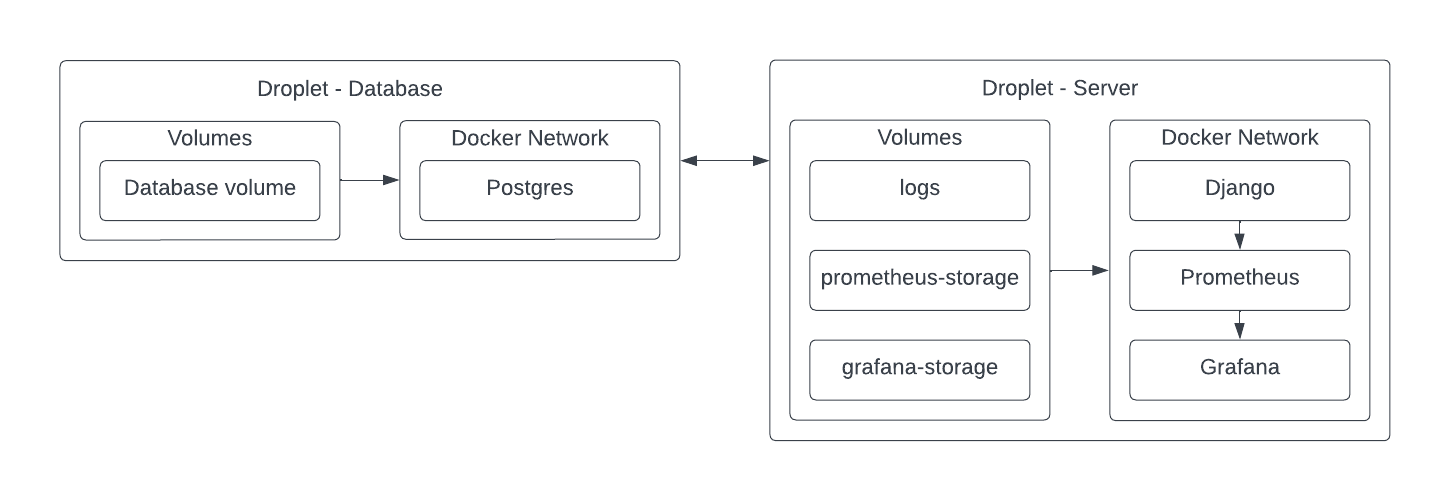
\includegraphics[width=\textwidth]{images/system-architechture.png}
    \caption{Simplified system architecture}
    \label{fig:system-arch}
\end{figure}